%%%%%%%%%%%%%%%%%%%%%%%%%%%%%%%%%%%%%%%%%%%%%%%%%%%%%%%%%%%%%%%%%%%%%%
%     File: ExtendedAbstract_intro.tex                               %
%     Tex Master: ExtendedAbstract.tex                               %
%                                                                    %
%     Author: Andre Calado Marta                                     %
%     Last modified : 27 Dez 2011                                    %
%%%%%%%%%%%%%%%%%%%%%%%%%%%%%%%%%%%%%%%%%%%%%%%%%%%%%%%%%%%%%%%%%%%%%%
% State the objectives of the work and provide an adequate background,
% avoiding a detailed literature survey or a summary of the results.
%%%%%%%%%%%%%%%%%%%%%%%%%%%%%%%%%%%%%%%%%%%%%%%%%%%%%%%%%%%%%%%%%%%%%%

\section{Introduction}
\label{sec:intro}

Even after years of research, the brain remains to this day a mysterious information-processing biological system. The required number of degrees of freedom to perform a particular movement is typically much smaller than the ones made available by the muscular apparatus, thus yielding a redundant control problem with infinitely many possibilities. For example, the eye has six extra-ocular muscles (6 DOF), but to point the eye in any given direction, only two coordinates are needed. As it seems, the brain gradually tries to find the optimal control solution for a certain task, which was theorized by Nikolai Bernstein\footnote{N. Bernstein, “The Coordination and Regulation of Movements. Oxford : Pergamon Press,” 1967.}, yet it's unknown which cost is minimized: energy, speed or accuracy. The main topic of the ORIENT research project for the Lisbon team\footnote{\href{http://www.mbfys.ru.nl/~johnvo/OrientWeb/orient.html}{http://www.mbfys.ru.nl/~johnvo/OrientWeb/orient.html}} is to create an autonomous humanoid eye-head robot with foveal vision, realistic auditory inputs, three-dimensional nested eye and head motor systems, and rapid sensory-motor feedback control and learning algorithms. This robot will hopefully contribute to a better understanding of the eye's control system.\\

So far, a working mechanical model of a biologically inspired eye with six muscles has been built in a previous work \cite{tesemiguel}, shown in Figure \ref{cha1:sec1:fig:curr_eye_model}. Currently, it is using an Inertial Measurement Unit (IMU) to estimate the eye's orientation. Although these units are good on acceleration and velocity measurements, they tend to have a significant position drift when determining the orientation. This work focuses on studying whether the addition of a camera to the system, could lead to a more precise and stable estimate for the orientation of the eye.\\

\begin{figure}[ht]
	\centering
	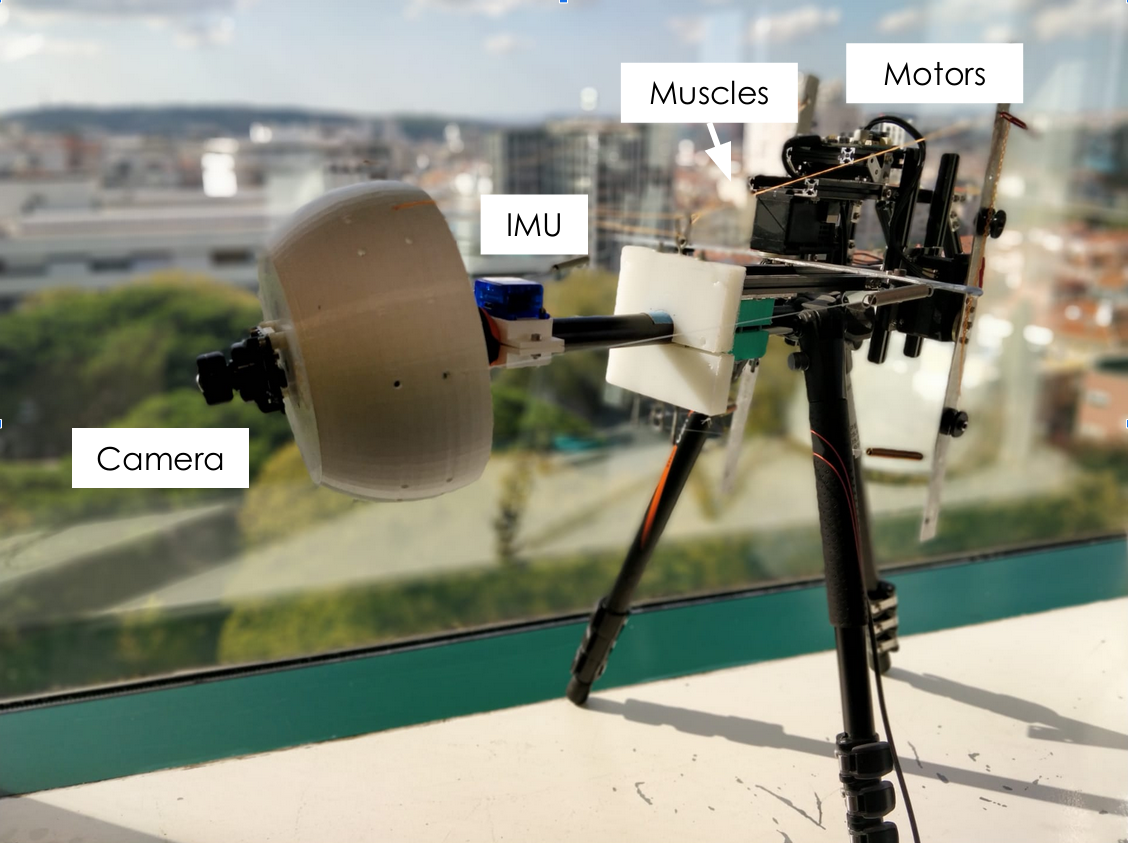
\includegraphics[width=0.4\textwidth]{images/prototypenew.png}
	\caption{The current mechanical eye model. It is composed of an IMU, seen on the middle of the image, and connected to a white eye ball enclosure mounted on a spherical joint, in turn connected to six elastics, representing the eye muscles, and finally controlled by three motors that pull at those elastics (paired by the aluminum strips). The three motors are controlled by the computer. The embedded camera is seen on the left.}
	\label{cha1:sec1:fig:curr_eye_model}
\end{figure}

The eye model will eventually rely on accurate camera output, so to foster a solid neuroscientifically inspired study with this model, it's indispensable to have the best possible estimates of the camera's orientation, as well as to consider the computational speed versus accuracy trade off for real-time operations. The accuracy and computational time mainly depend on the complexity of detecting correspondences between consecutive images and on the algorithm responsible for calculating the camera's orientation difference between those images. 
There is a long literature on estimating the orientation of a camera from natural visual features. However, the current prototype, has a peculiarity. There is a translation movement associated to the camera movement that may be defined as a function of the rotation and the length from the camera's center to the rotational center (spherical joint) that holds the camera. That length is referred to as baseline. Hence, the main goal  is to identify the algorithm that does the job best under this constraint. Beyond that, this work also aims to (i) understand how much  accuracy can be gained from using the constraint versus the classical unconstrained or rotation-only approaches, (ii) how the algorithms behave in the real world and (iii) evaluate the improvement of using the camera over the IMU.



